RGG ships AssyGen and CoreGen from Meshkit 1.2 \footnote{See \url{http://trac.mcs.anl.gov/projects/fathom/wiki/MeshKit}}.  RGG allows you to provide paths to Cubit\footnote{See \url{https://cubit.sandia.gov/}.}.

\section{Add Paths to Preferences}

In order for RGG to mesh an INP file, we utilize AssyGen, CoreGen, and Cubit.  On Linux and Mac, we package Assygen and CoreGen with RGG.  However, RGG needs an external Cubit for meshing.  RGG will look for Cubit 13.1 in the normal location.  However, we provide a means to manually set Cubit and also point to a different AssyGen and CoreGen than what is shipped.

Access the \ui{system preferences window} by clicking on the \ui{edit menu} of the \ui{toolbar} on Linux and Windows.  On Mac, click on the \ui{preferences item} of the \ui{RGG Nuclear menu}.

This brings up the \ui{system preferences window}.  By default, we use the packaged AssyGen and CoreGen, so we only provide a section to set Cubit (Figure \ref{fig:prefDefault}).  By checking ``Use Custom Meshkit," one is provided sections to direct RGG toward the desired AssyGen/CoreGen (Figure ~\ref{fig:prefCustom}).  To add one, click the \ui{browse button} in the section that corresponds to the desired executable.  Locate the executable and click the \ui{open button} to get back to the system preferences window.

\begin{figure}
\centering
\begin{subfigure}{.5\textwidth}
  \centering
  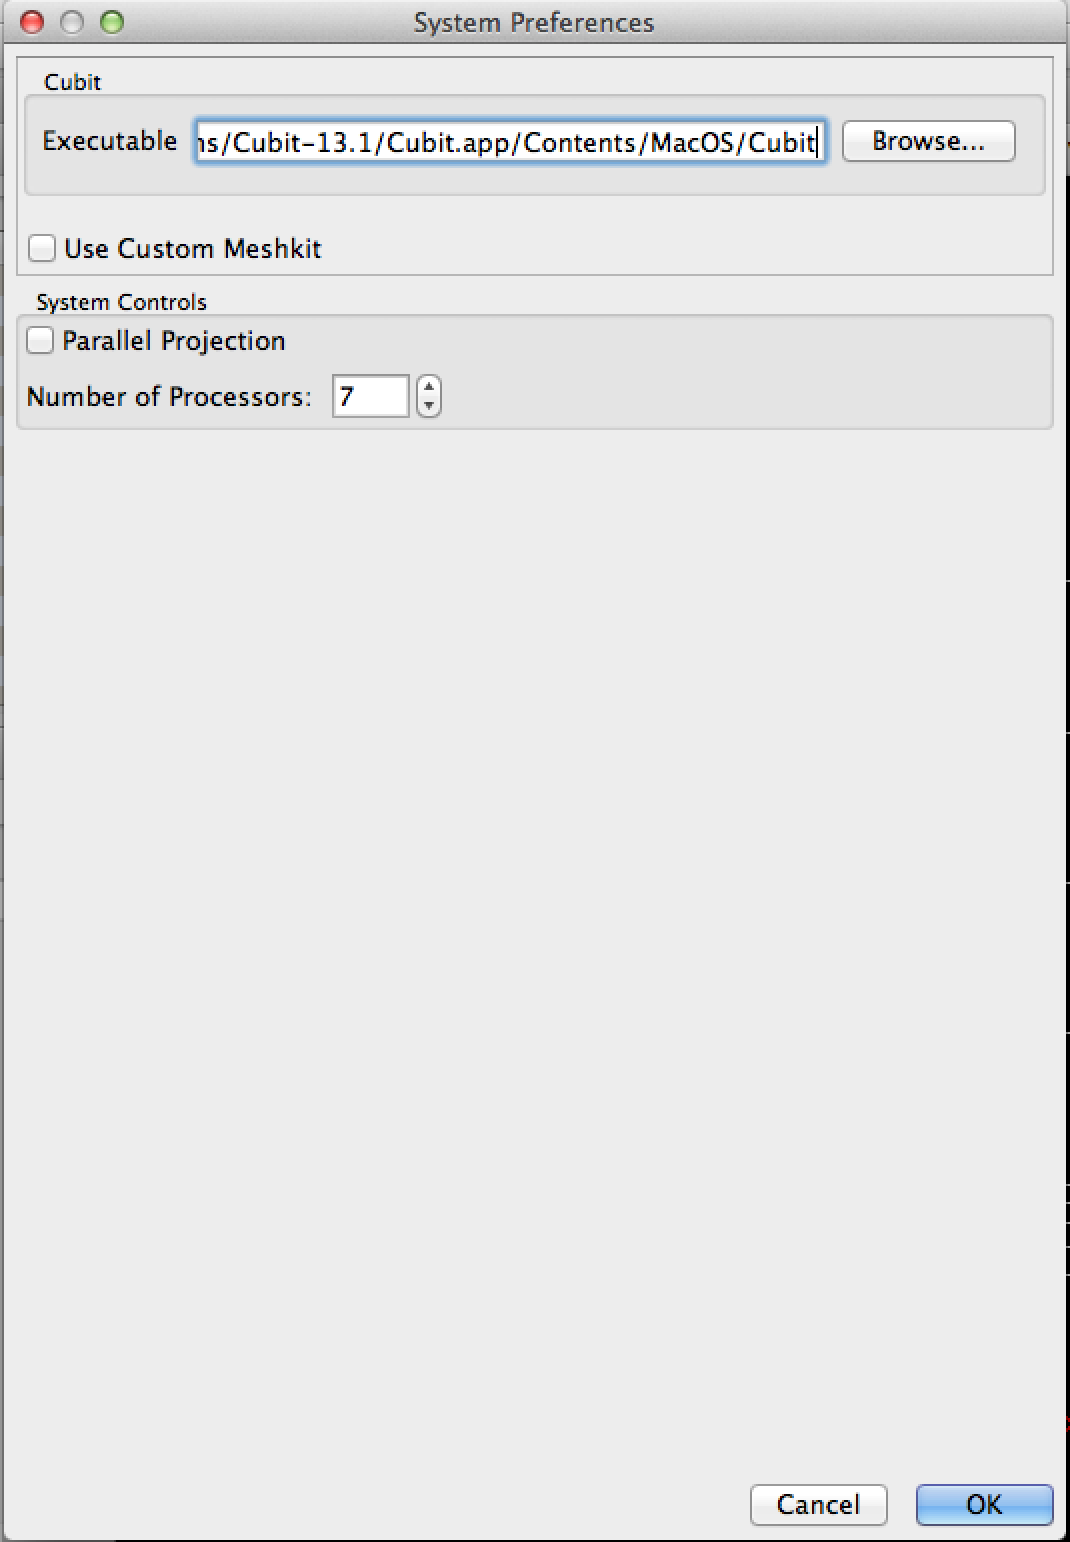
\includegraphics[width=0.6\linewidth]{Images/packaged_meshkit.png}
  \caption{Using packaged AssyGen/CoreGen}
  \label{fig:prefDefault}
\end{subfigure}%
\begin{subfigure}{.5\textwidth}
  \centering
  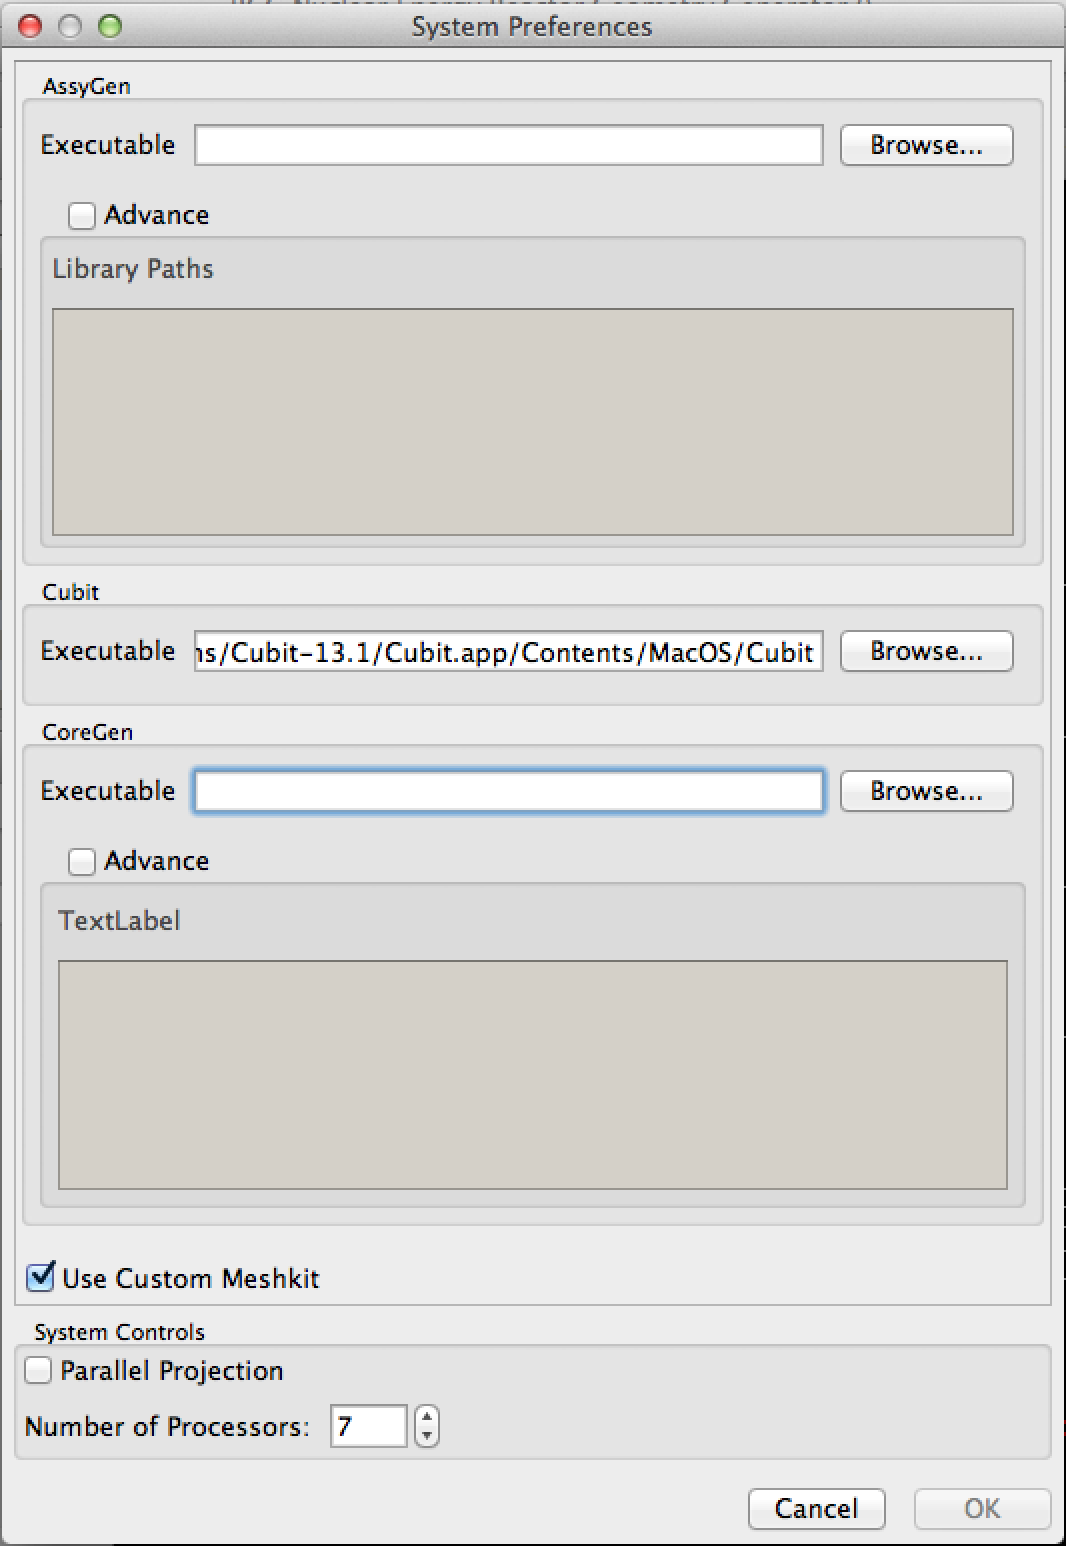
\includegraphics[width=0.6\linewidth]{Images/custom_meshkit.png}
  \caption{Provide a custom AssyGen/CoreGen}
  \label{fig:prefCustom}
\end{subfigure}
\caption{Configuration of meshing executable.}
\label{fig:configOptions}
\end{figure}

Note the \ui{advance checkbox} in the AssyGen and CoreGen sections.  If either of these executables require shared libraries in non-standard locations, you can click this checkbox to activate the \ui{library paths text box}.  You can specify directories where the shared libraries are, with each line being another location.

We also run multiple AssyGen and Cubits in parallel decrease the wait time for a mesh.  The number of parallel jobs is controlled by ``Number of Processors."